%!TEX root = ../thesis.tex
%*******************************************************************************
%****************************** Third Chapter **********************************
%*******************************************************************************

\chapter{Matherial and methods}
\label{chap:matherial_methods}
\ifpdf
    \graphicspath{{Chapter3/Figs/Raster/}{Chapter3/Figs/PDF/}{Chapter3/Figs/}}
\else
    \graphicspath{{Chapter3/Figs/Vector/}{Chapter3/Figs/}}
\fi


\section{Constitution du benchmark} % (fold)
\label{sec:constitution_du_benchmark}

\victor{données specifiquement utilisées}

\victor{simulateur rapide}


\victor{TODO : nuisance parameters}
\victor{TODO : importance weight}


\section{Evaluation metric} % (fold)
\label{sec:evaluation_metric}

Many methods to estimate the parameter of interest and its variance are available.
If changing the set of hyper parameter for the learning procedure is considered as changing the method then countless methods are to be evaluated.
Automating the measure of the performances of a proposed method is crucial to select the best method.
In this section is described a simple but general procedure to measure the performances of a given method.

The usual criterions to evaluate an estimator $\htheta$ are the bias, the variance and the mean squared error defined as follow :
\begin{equation}
  Bias(\htheta) = \EE[\htheta] - \thetas
\end{equation}
\begin{equation}
  Var(\htheta) = \EE[ (\htheta - \EE[\htheta])^2 ] = \EE[\htheta^2] - (\EE[\htheta])^2
\end{equation}
\begin{equation}
  MSE(\htheta) = \EE[(\htheta - \thetas)^2] = Var(\htheta) + [Bias(\htheta)]^2
\end{equation}

To evaluate these criterion we need to repeat the experiement $N$ times leading to many estimation of the parameters $\hmu^{(k)}$ and $\hshmu^{(k)}$.
Repeating the experiment can be done through cross-validation methods.


\subsection{Evaluation of the parameter of interest estimator} % (fold)
\label{sub:evaluation_of_the_parameter_of_interest_estimator}

First, let's focus on evaluating the estimator of the parameter of insterest $\hmu$.
The true value of $\mu$, noted $\mus$, is available during tests since it is an input of the simulator.

From the estimation of its expected value
\begin{equation}
  \EE[\hmu] \approx <\hmu^{(k)}>_k = \frac{1}{N} \sum_{k} \hmu^{(k)}
\end{equation}
it is possible to estimated the criterions

\begin{equation}
  Bias(\hmu) \approx <\hmu^{(k)}>_k - \mus
\end{equation}
\begin{equation}
  \label{eq:var_hmu}
  Var(\hmu) \approx <\hmu^{(k)} \times \hmu^{(k)}>_k - (<\hmu^{(k)}>_k)^2
\end{equation}
\begin{equation}
  MSE(\hmu) = Var(\hmu) + [Bias(\hmu)]^2
\end{equation}

\subsection{Evaluation of the variance estimator} % (fold)
\label{sub:evaluation_of_the_variance_estimator}

The evaluation of the variance estimator $\hshmu$ could be done in the same way if the true variance $Var(\hmu)$ can be computed.
If this is not the case an approximation is available using \autoref{eq:var_hmu}.

\begin{equation}
  Bias(\hshmu) \approx <\hshmu^{(k)}>_k - Var(\hmu)
\end{equation}
\begin{equation}
  Var(\hshmu) \approx <\hshmu^{(k)} \times \hshmu^{(k)}>_k - (<\hshmu^{(k)}>_k)^2
\end{equation}
\begin{equation}
  MSE(\hmu) = Var(\hshmu) + [Bias(\hshmu)]^2
\end{equation}



\section{"Domain adaptation"} % (fold)
\label{sec:domain_adaptation}

\victor{Tangent prop}

Tangent Propagation is learning to become robust to a known geometrical/differentiable transformation of the input features.

\victor{how Pivot is "domain adaptation"}

Pivot network are trained to become robust to the variation of a known feature (which may not be an input feature).


\section{More direct approach} % (fold)
\label{sec:more_direct_approach}

\victor{INFERNO}


\topic{This method is inspired from mixture density networks, inferno and neural statistician. 
Other solutions to the inverse problem includes ABC, VI and probabilistic programming.}


\subsection{Regression} % (fold)
\label{sub:regression}

\topic{A simple but efficient solution is to map the input data to the target with a neural network whose architecture and training procedure are carefully chosen.}
\subsubsection{Setting}
\topic{Although the generator is available classical Bayesian inference is difficult because of the intractable likelihood.}

A generative model $G(\theta)$ is available to simulate the studied process and retrieve the observations $x$ from given parameters $\theta$.
The objective is to reverse the generator $G^{-1}(x)$ to access the quantities of interest ruling the process.

Since the process is stochastic the generator can produce different observations from the same parameters.
The probability of observing $x$ if the generator is fed with $\theta$ is $p(x | \theta)$.
Therefore reversing the generator means finding $p(\theta | x)$.
From Bayes theorem we get :

\begin{equation}
    p(\theta | x) = \frac{p(x | \theta) p(\theta) }{p(x)}
\end{equation}
Unfortunately the likelihood $p(x | \theta)$ is often intractable because of high dimensional integrals.
To avoid this pitfall the posterior $p(\theta | x)$ is approximated by a tractable distribution $q_\phi(\theta | x)$.


\subsubsection{Density network}

\topic{Mixture density networks are a tractable but powerful tool to approximate a conditional probability density.}

A way of approximating the posterior $p(\theta | x)$ is to define a tractable but flexible enough family of distribution $q_\phi(\theta | x)$ parametrized by $\phi$.

Initially introduced in \cite{Bishop94mixturedensity} as a generalization of least square methods to train neural network, mixture density networks (MDN) can be made as powerful as one require while staying tractable and allowing to estimate the uncertainties of the predictions.

The target density is approximated by a linear combination of kernels $k$ :

\begin{equation}
    q_\phi(\theta | x) = \sum_{i=0}^K m_i(x ; \phi) k_i(\theta | x ; \phi)
\end{equation}
where $m_i(x ; \phi)$ are the mixture coefficient
and the kernels $k_i(\theta | x ; \phi)$ usually taken as Gaussian :
\begin{equation}
    k_i(\theta | x ; \phi) = \frac{1}{\sigma_i(x ; \phi) \sqrt{2 \pi}} e^{- \frac{1}{2} \left ( \frac{\theta-y_i(x ; \phi)}{\sigma_i(x ; \phi)} \right )^2} 
\end{equation}

$m_i(x ; \phi)$, $\sigma_i(x ; \phi)$ and $y_i(x ; \phi)$ are the outputs of a neural network, whose parameters are gathered in $\phi$, and taking the data as input.
Finally, the mixture coefficient have to sum up to 1.
\begin{equation}
    \sum_{i=0}^K m_i(x ; \phi) =  1
\end{equation}

The motivation for this approximation is twofold.
First, given enough well chosen parameters a Gaussian mixture model can approximate any density.
Second, a neural network with enough hidden unit is able to approximate any continuous function with arbitrarily precision.
Combining these two properties leads to an arbitrarily powerful approximation of any conditional density $p(\theta|x)$ given enough resources.

The neural network parameters $\phi$ can then be obtained by maximizing the likelihood that the model produced the given data.

\begin{equation}
    \phi^\star = \argmax_\phi \mathcal L (\phi)
\end{equation}
\begin{equation}
    \mathcal L (\phi) = \sum_{i=0}^K m_i(x ; \phi) k_i(\theta | x ; \phi)
\end{equation}

Similarly to training a regular neural network regressor with least square, MDN's training is supervised.
Therefore requires data for which the ground truth is available which is verified in our case.

Finally the likelihood, with Gaussian kernels, is fully differentiable making possible the use of stochastic gradient descent methods to obtain the neural network parameters $\phi$.

\subsubsection{Training}

\topic{MDN are trained like classical regressor and allow to compute the uncertainty of the predictions.}

The parameters $\phi$ are obtained by maximizing the likelihood :
\begin{equation}
    \phi^\star = \argmax_\phi \mathcal L (\phi)
\end{equation}
For convenience the optimization is usually turned into a minimization of the negative log likelihood (NLL) :
\begin{equation}
    \phi^\star = \argmin_\phi - \log \mathcal L (\phi)
\end{equation}

In the simple case of one Gaussian component ($K=1$) the NLL is :
\begin{equation}
    \phi^\star = \argmin_\phi \left\{ \log(\sigma(x;\phi)) + \frac{1}{2}\log(2\pi) + \frac{(\theta - y(x;\phi))^2}{2\sigma(x;\phi)^2} \right\}
\end{equation}

The learning procedure is supervised since we need both observed data $x$ and the associated value for  $\theta$.

Since the likelihood is fully differentiable in $\phi$, the optimization can be solved using stochastic gradient descent methods.

\begin{algorithm}[H]
 \For{$i \in [0, N]$}{
  $\theta_i$    $\gets$ sample from $p(\theta)$ \;
  $x_i$      $\gets$ $G(\theta_i)$ \;
  $m_i, y_i, \sigma_i$ $\gets$ $f(x_i; \phi_i)$ \;
  $loss_i$   $\gets$ $-\log \mathcal L(\phi_i; m_i, y_i, \sigma_i)$ \;
  $grads_i$  $\gets$ backward($loss_i$) \;
  $\phi_{i+1}$ $\gets$ Optimizer($\phi_i$, $grads_i$) \;
 }
 \caption{Training procedure}
\end{algorithm}

As long as a flexible and powerful enough parametric differentiable function is mapping the data $x$ to the parameter $\theta$ it is possible to approximate the conditional density.
Once trained the inference is straightforward.
From the experimental data $x^\star$ the mean and variance can be easily extracted:

\begin{align}
    \bar \theta & = \mathbb E_{p(\theta | x^\star)}[\theta] \\
    & \approx \mathbb E_{q_\phi(\theta | x^\star)}[\theta] \\
    & = \sum_{i=0}^K m_i(x^\star ; \phi) \int d\theta ~ \theta ~ k_i(\theta | x^\star ; \phi) \\
    & = \sum_{i=0}^K m_i(x^\star ; \phi) y_i(x^\star ; \phi)
\end{align}

\begin{align}
    \Delta\theta^2 & = \mathbb V_{p(\theta | x^\star)}[\theta] \\
    & \approx \mathbb V_{q_\phi(\theta | x^\star)}[\theta] \\
    & = \sum_{i=0}^K m_i(x^\star ; \phi) \int d\theta ~ \theta^2 ~ k_i(\theta | x^\star ; \phi) - \bar \theta^2 \\
    & = \sum_{i=0}^K m_i(x^\star ; \phi) \left [ \sigma_i(x^\star ; \phi)^2 + y_i(x^\star ; \phi)^2 - \bar \theta^2 \right ]
\end{align}

\subsubsection{Neural network architecture}
\topic{Details about the neural network architecture for MDN with importance weighted dataset as input}

In order to accurately capture the complex mapping between the data and the parameters the architecture of the neural network should embody the constraints of the chosen family distribution.

The requirement that the mixture coefficients $m_i$ sum up to 1 is enforced using softmax operator on the $K$ output neurons representing the $m_i$.
Similarly the standard deviation of Gaussians should always be strictly positive which is fulfilled by interpreting the neuron output as $\log(\sigma_i)$.
No particular operation are necessary on the mean $y_i$ of the Gaussians since it can take whatever real value.

If the studied process is stochastic the observations are usually composed of repeated independent measurements of an event.
Then the observable is not a real valued vector $x \in \RR$ but a set of data points $D = \{v_i \in \RR \}_{i=0}^N$.
The output is still a real valued vector meaning that the neural network architecture should include some reduction function to map the set of vector to a single vector.
Usual candidates are averages, minima, maxima, products, sums, geometric means or others that reduce the dimension and remain invariant to the input order of the input vectors.
In practice the average is the favorite one.

When the studied process includes some very rare events the simulation uses importance sampling. 
The simulation output includes importance weights to allow many rare events to be produced while keeping the distribution of events similar to reality.
The neural network must take into account the importance weights to accurately regress the parameters.
Which leads to use weighted average instead of simple average for example.

More precisely, for 2 datasets $D$ and $D^\prime$ if the associated empirical distribution are equal then the neural network output should also be equal.

\begin{equation}
    \forall x, p_D(x) = p_{D^\prime}(x) \implies f(D; \phi) = f(D^\prime; \phi)
\end{equation}

with,
\begin{equation}
    p_D(x) = \sum_{v \in D} w_i \delta (x - v)
\end{equation}
and $\delta$ is the Dirac distribution function.

\victor{Oui mais Quid du fait que l'incertitude dépend du nombre d'évènement ? $\sigma$ doit changer si j'ai 10 fois moins d'évènements, non ? Oui mais d'un autre coté le réseaux est conçu pour pouvoir extraire la variance des observables d'entrée donc il peut gérer ça tout seul... Aussi si on a 10 fois moins d'évènement la distribution empirique n'est pas du tout la même donc c'est pas pertinent !}


\topic{Neural network using reduction function, such as the average, can extract complex link between the parameters of a generative distribution and a dataset which is a realisation of this distribution.}

Section 7 of \cite{lucas:hal-01791126} gives a proof that the given \emph{"permutation invariant neural networks"} architecture is a universal approximator.



\subsubsection{Nuisance parameters}
\topic{Nuisance parameters are marginalized using Monte Carlo integral approximation.}

The objective is to infer the parameter $\mu$ of a model that describes a stochastic system from experimental data $D$.
However $\mu$ alone is not enough to describe the experimental data.
More causal parameters, noted $\alpha$, are required.
Since the parameters $\alpha$ are not the object of study they are tagged as \emph{nuisance} parameters in opposition to the parameter \emph{of interest} $\mu$.

The nuisance parameters have to be marginalized.
\begin{equation}
    p(\mu | x) = \int d\alpha ~ p(\alpha | x) ~ p(\mu | x, \alpha)
\end{equation}

This integral can be approximated with Monte Carlo.

\begin{equation}
  \int d\alpha ~ p(\alpha) ~ f(\alpha)
  \approx \sum_i w_i ~ f(\alpha_i)
\end{equation}

Where $p(\mu | x, \alpha)$ is approximated using a trained MDN as seen previously.
The neural network $f$ produces the mixture parameters $m_i, y_i, \sigma_i$ from the experimental data $x^\star$ and sampled $\alpha$.

\begin{algorithm}[H]
 \For{$i \in [0, N]$}{
  $\alpha_i, w_i$ $\gets$ MC sample from $p(\alpha)$ \;
  $m_j, y_j, \sigma_j = f(x^\star, \alpha; \phi^\star)$ \;
  $\bar\mu = \sum_{j=0}^K m_j y_j $ \;
  $\Delta\mu = \sum_{j=0}^K m_j \left [ \sigma_j^2 + y_j^2 - \bar \mu^2 \right ]$ \;
  $\hat\mu$  $\gets$ $\hat\mu + w_i \times \bar\mu$ \;
  $\hat\sigma$  $\gets$ $\hat\sigma + w_i \times (\bar\mu^2 + \Delta\mu^2)$ \;
 }
$\hat\sigma$  $\gets$ $\hat\sigma - \hat\mu^2$ \;
\caption{Marginalizing the nuisance parameters $\alpha$ using MC to compute the integral.}
\end{algorithm}


\subsubsection{Discussing the related work} 

Using a neural network to directly map the dataset to the estimated parameter distribution can be viewed as an extension of the work done in INFERNO \cite{DECASTRO2019170inferno}. 
Indeed the current state of the art is using a classifier score histogram to produce summary static while INFERNO includes the summary statistic production in the neural network.
In this work the next step, maximum likelihood fit to retrieve the parameter of interest, is also left to the neural network.

Neural Statistician \cite{Edwards17neuralstatistician} is also relying on a similar neural network architecture to compute summary statistics.
The idea in Neural Statistician is that similar datasets can be gathered as originating from the same generative model including a global parameter to control the shift between domains.
In this work the architecture is slightly improved to take into account importance weights.
Moreover the objective is completely different since we consider supervised regression.

Causal parameters are often related to properties of the distribution of the data in statistical simulations.
The architecture should reflect this link in order for a neural network to capture the relevant information.
This work is using Mixture density network \cite{Bishop94mixturedensity} combined with neural network architectures design to learn summary statistics on datasets.
Such architecture is shown in \cite{Edwards17neuralstatistician}, in the context of transfer learning and one shot learning, where the neural network is producing summary statistics to embed the link between similar datasets.
\cite{DECASTRO2019170inferno} is the closest work of this study in which the authors optimize a neural network to produce of summary statistics that reduces the uncertainty on the parameters of interest estimation.


\victor{TODO : related to Amortized VI ? Related to simple Gaussian fit ?}


\subsection{Toys} % (fold)
\label{sub:toys}

\victor{Montrer sur des toys}

\subsubsection{Apple and pears}

Let's start with a toy problem and make it gradually more complex.
The study is about finding the proportion $\mu$ of apples and pears in a bag.
The only information available is the total number of fruits in the bag and the weight of each individual fruit.
Apples and pears weights are normally distributed and slightly different.
The dataset is a set of real values $D = \{ x_i \in \RR \} $

From the average weight of the fruits in the bag a linear regression is enough to find the link between $D$ and the parameter of interest $\mu$.
The model can be trained if enough bags in which the proportion is known is available for training.
This simplicity is wanted to test the method.

Since the weight of a fruit is stochastic, two bags of fruits with the same number of apples and pears may have a different average weight.
Leading to some uncertainty in the predicted proportion that must be reported.


\victor{VAE}




\begin{figure}[htb]
  \centering
  \begin{subfigure}[t]{0.49\linewidth}
    
\includegraphics[width=\linewidth]{minion}
    \caption{Minions}
    \label{fig:minion}
  \end{subfigure}%
  \hfill
  \begin{subfigure}[t]{0.49\linewidth}
    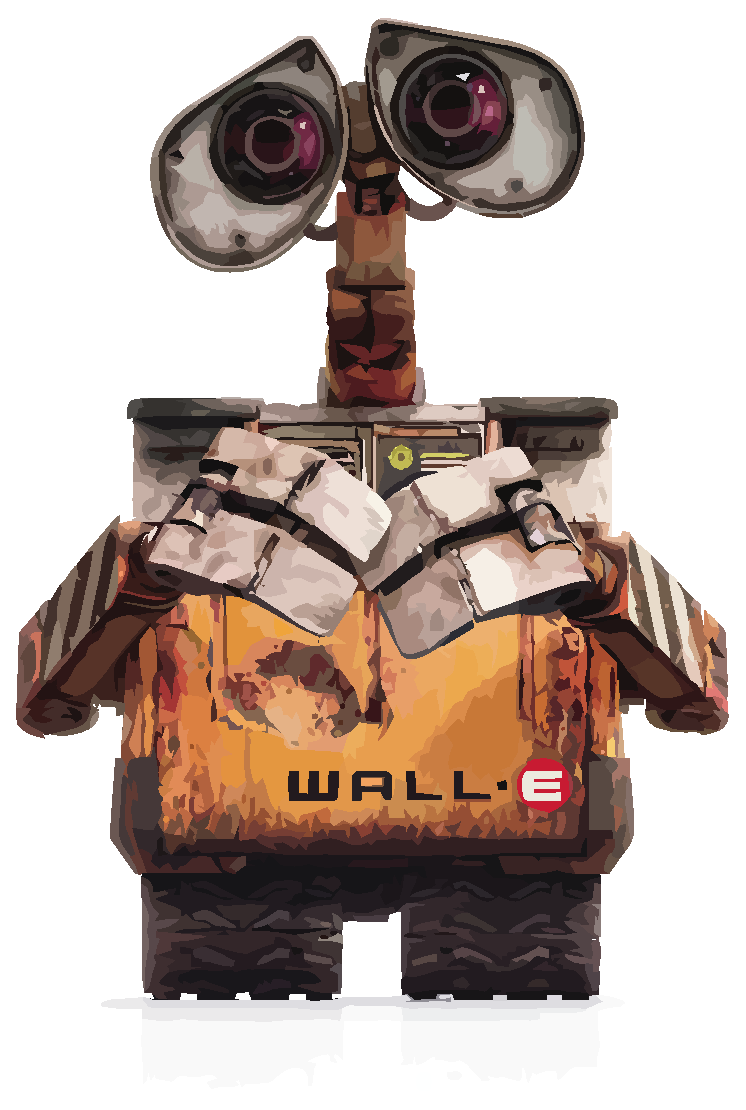
\includegraphics[width=\linewidth]{WallE}
    \caption{"Eve"}
    \label{fig:walle}
  \end{subfigure}
  \caption{Comparison Minions (left) and WallE (right)}
  \label{fig:comparision}
\end{figure}
